\documentclass[12pt]{jpconf}
%\documentclass[10pt, landscape, twocolumn]{article}

\usepackage{graphicx}
\usepackage{amsmath, amssymb}

%\usepackage{tikz}
\usepackage{caption}

\usepackage{xcolor}
\definecolor{amaranth}{rgb}{0.9, 0.17, 0.31}
\definecolor{amethyst}{rgb}{0.6, 0.4, 0.8}
\definecolor{ao}{rgb}{0.0, 0.0, 1.0}

\usepackage{tikz}
\usetikzlibrary{arrows}

\begin {document}
\title{Application of convolutional neural networks in optical text recognition to junk data filtering}
\author{Razumov T.E.$^{1,2}$, Churikov D.V.$^{2,3}$, Kravchenko O.V.$^{2-4}$}

\address{
$^1$\,Mail.ru Group, Leningradsky pr., 39--79, Moscow, 125167, Russian Federation\\
$^2$\,Scientific and Technological Centre of Unique Instrumentation, Butlerova str., 15, Moscow, 117342, Russian Federation\\
$^3$\,Kotel'nikov Institute of Radio Engineering and Electronics of RAS, Mokhovaya st. 11--7,
Moscow, 125009, Russian Federation\\
$^4$\,Federal Research Center ``Computer Science and Control'' of RAS, Vavilova st., 40, Moscow, 119333, Russian Federation
}

\ead{timofey.razumov@corp.mail.ru}


\begin{abstract}
	In this paper, the problem of constructing a model for detecting and filtering unwanted spam messages is solved. A fully connected convolutional neural network ({FCNN}) was chosen as the model of the classifier of unwanted emails in email. It allows you to divide emails into two categories: \emph{spam} and \emph{not spam}.
	The main result of the research is a software application in the \textsf{C++} language, which has a micro-service architecture, and solves the problem of image classification. The app is able to handle more than $10 ^ 6 $ requests per minute in real time.
\end{abstract}

% --------------------
\section{Introduction}
Presently, the amount of information produced by humanity
is growing exponentially. Significant benefits can be derived from this information only if the data is properly processed and analyzed.
On the other hand, the actual task of data processing in general is the task of junk data filtering and it transforms into the task of spam messages filtering in case of IT technologies particularly.
The latter is due to the fact that the exchange of information of various information by default uses email. It's one of the cheapest, easiest to use, most easily accessible, official, and most reliable way to communicaty nowadays.
Junk data or spam messages, generally speaking, may contain heterogeneous test--visual information. Modern deep
learning algorithms are used to analyze emails traffic with various information received in real time \cite{Makkar2021}.
In this case, first features (characteristics) are extracted from the image, and then a decision is made.
Another approach is a classification one that include the support vector machine algorithm and the random forest method. These methods for solving the problem of filtering spam messages are compared in \cite{Taylor2020}.
At the same time, filtering algorithms are usually stochastic \cite{Garg2021} and are used in combination with optimization techniques for some objective function. Various probabilistic models are used to solve the problem of email classification. One of the most commonly used approach is the naive Bayesian classifier. Other one is the particle swarm method is one of the numerical methods of stochastic optimization and it is used in data filtering problems, since it is not necessary to specify an analytical expression of the gradient of the optimized function. The particle swarm method refers to stochastic optimization methods and it is utilized for heuristic global optimization of the parameters of a naive Bayesian classifier. A complex approach using the naive Bayes algorithm together with the particle swarm optimization method was applied in \cite{Parmar2020}.
The evolutionary model of spam classification is also presented in \cite{Mohammad2020}.

The problem of detecting and filtering unwanted spam messages is investigated in present paper. A fully connected convolutional neural network ({FCNN}) is considered as a solution tool, which was chosen to classify junk email messages.


\section{Methodology}
\subsection{Statement of the problem}
Let's consider a set of objects $ X = X_L \cup X_T$, where
$X_L$ is training sample,
$X_T$ is test sample,
$Y$ is set of valid responses. Also, assume that there is an objective function $g: X \rightarrow Y$, whose values are known only on the set $X_L$. Let the data be distributed according to some unknown distribution $P (x,y) = P(x) P (y|x)$, with some loss function given
$$
R(g(x), y) = 
\begin{cases} 
\phantom{>}0, & y = g(x), \\
> 0, & y \neq g(x).
\end{cases}
$$
In accordance with the principle of minimizing empirical risk, the loss function is used to be minimazied. In other words a decision function $g(x)$, which on average will lead to the smallest error is determined. Formally, one need to solve the minimization problem as follows
$$
g(x) = \operatorname*{argmin}_{f: X \rightarrow Y} E_{X,Y} R(f(x), y).
$$
To state the problem of junk data filtration, the set $Y$ consists of two elements $\{0, 1\}$, where $0$ and $1$ are desirable and undesirable data, respectively. Due to the roughness of the discrete computing methods $R = P[0, 1]$ is usually used in practice. Thus, the result of the classifier $r' = r(x)$ belongs to the desired class with a given threshold probability $\alpha$, which minimizes the error of the first and second kind.

\subsection{Requirements for the solution}
Since, the speed of the information traffic increases an additional important requirement on the speed of the model and the system as a whole is imposed. The time for checking a single message should not exceed $\leqslant3$ seconds, which imposes additional constraint on the tools utilized and on the fault tolerance of the entire system.
From the moment of receiving the message to the moment of making a decision about its type the text information goes through three stages of processing are shown in figure\,\ref{fig:00}.
\begin{figure}[h!]
\centering
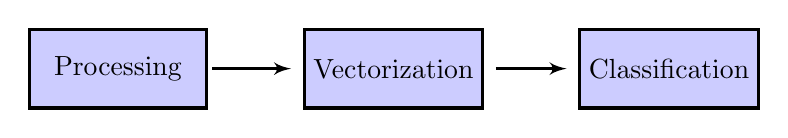
\begin{tikzpicture}
\draw (0.0,0) node[rectangle, line width=1.15pt, fill=blue!20, minimum height=1cm, minimum width=2.25cm, draw] {Processing};

	\draw (3.5,0) node[rectangle, line width=1.15pt, fill=blue!20, minimum height=1cm, minimum width=2.25cm, draw] {Vectorization};

\draw (7.0,0) node[rectangle, line width=1.15pt, fill=blue!20, minimum height=1cm, minimum width=2.25cm, draw] {Classification};

\draw[-latex', line width=1.15pt] (1.20,0) -- (2.20,0);

\draw[-latex', line width=1.15pt] (4.80,0) -- (5.70,0);

\end{tikzpicture}
\caption{\label{fig:00}Stages of the text processing.}
\end{figure}

\subsection{Text processing}
Since the text has a very heterogeneous structure and a single word can be written in many different ways (different font, encoding, case, etc.), but still have the same meaning, different methods of tesxts preprocessing or combination of them are considered.

The first step of preprocessing is to parse the text and decode it into the specified encoding. Then it is conversed to the lower (or upper) case, unnecessary spaces and indents are removed. The characters are replaced according to the specified rule. Further, some methods of text processing are introduced below.

\subsubsection*{Stop words.}
The text often contains many characters that don't have any semantic sence for the general meaning (two spaces, paragraph indentation).
Similarly, stop words are the words in any language that don't have much sence in a sentence. Often, stop words include punctuation marks, pronouns, and prepositions. Often, spammers use them to make texts noisy in order to hide the spam content of the message. Since they can be safely ignored without sacrificing the meaning of the sentence, classification tasks often resort to removing them from the original message.

\subsubsection*{Stemming and lemmatization.}
Usually texts contain different grammatical forms of the same word, and may also contain the same root words. Using different algorithms, lemmatization and stemming aim to reduce all occurring word forms to a single, normal dictionary form.

Stemming is a crude heuristic process which cuts off ``extra'' from the word root, often resulting in a loss of word--formation suffixes. The main problem encountered when using stemming is the processing of words which, when forming different grammatical forms, change not only the ending, but also the base of the word. To minimize the negative consequences of too aggressive truncation of words by the streamer, it is necessary to perform memming of the searched keyword, and then compare the result with the output of the streamer for each of the words in the processed text. 

Lemmatization is a more subtle process, which uses dictionary and morphological analysis to reduce a word to its canonical form (lemma). However, it applies simplistic word analysis without considering the context. This leads to ambiguities in determining parts of speech. This ambiguity cannot be resolved without involving the morphological analyzer.

Basically, lemmatization gives the most accurate results, and it is utilized in the proposed approach.

\subsection{Text vectorization}
Modern machine learning algorithms are not able to process raw text directly, so it is necessary to develop a map from text to a vector space. This is called feature extraction. 
Let's consider several approaches allows to construct this map below.

\subsubsection*{Bag of words.}
The ``bag of words'' (BOW) model is a simplified representation of the text that used in natural language processing and information retrieval problems. Text is considered as a bag (multiset) of words or phrases in the case of combinations of terms. Grammar is ignored as well as even words order in some cases, but multiplicity is preserved in BOW. Each term (word or phrase) is assigned with a number. Then, text is defined by the vector $x=(x_1,..., x_N)^T$, where $N$ is the dimension of the finite dictionary $X_L$ contains the unique terms of the training sample. Several options to define $x_i$ are possible, such as
\begin{enumerate}
\item Boolean weight equals $1,$ if element exists in a message or 
$0,$ else.
\item The number of occurrences of the $i$--th term in the text is 
$x_i = n_i.$
\item Term frequency is $x_i = n_i\slash\left(\sum\limits_{k=1}^i n_k\right).$
\end{enumerate}
Third option was chosen to perform better convergence rate.

\subsubsection*{Word2Vec.}
The main problem of BOW model is the loss of context between words. Since in natural language, the permutation of even two words of a sentence can completely change the meaning, this classification approach may have low accuracy.
Word2Vec is a text vectorization tool that takes into account the contextual relationship between words. The algorithm is based on huffman binary tree, skip--gram, negative sampling approaches. The bottle-necked place in Word2Vec is to find the context for the rare words.

\subsubsection*{Fast Text.}
FastText is a Word2Vec extension proposed by Facebook in 2016 \cite{Mikolov2013,Bojanowski2017}. Fast Text approach splits the words into several $n$--grams (proverbs) Instead of considering individual words as an input of a neural network. After training the neural network, the embedding words for all $n$--grams from the training dataset arise.
Applying such an approach, the solution becomes more sensitive to rare words, since it is highly likely that some of their $n$--grams are also presented in other words. Training the Fastext model takes longer time, but it works more precise than Word2Vec and allows to  represent rare words correctly.

\subsection{Text classification}
After text vectorization, a transform from a set of features to a set of classifiable objects $g: X \rightarrow Y$ is developed.
According to the article \cite{Bommannavar2014,Yang2014}, unique points were marked by bins and the optimal threshold accuracy $\alpha = 0.75$ was calculated, which provides optimal pressision and recall for our model and minimizes the error variance.

\subsubsection*{Logistic regression.}
The common approach in the classification is to apply the logistic regression method
$$
g(x) = \left(1 + \exp{ \left( \sum_{i=0}^n w_i x_i  \right) }\right)^{\!\!-1}\!\!\!\!,
$$
where $\mathbf{w}=(w_1,\ldots, w_N)^T$ are weights of the model arised in training process.
Two different methods of text vectorization were examined experimentaly.
The results for BOW and Fast Text embeddings with logistic regression, are introduced in table\,\ref{tbl:01}.

\begin{table}[h!]
	\centering
	\caption{\label{tbl:01}Training result}
	\begin{center}
		\begin{tabular}{lll}
			\br
			embeddings & precision & recall \\
			\mr
			BOW & 0.91143 & 0.99961 \\ \hline
			Fast Text & \bf 0.95523 & \bf 0.89164 \\ 
			\br
		\end{tabular}
	\end{center}
\end{table}

\subsubsection*{Fully convolutional neural network (FCNN).}

The fully convolutional neural network with 3 layers was considered. A \textsf{ReLU} activation function was applied to the first and second layersthird, and the last one utilize \textsf{sigmoid} as an activation function. Data was regularized on each layer. Neural network can be defined as follows in our case
$$
g(x) = h_2 \left(\sum_{k=0}^{n_2} w''_k h_1\left(\sum_{j=0}^{n_1} w'_j h_0\left( \sum_{i=0}^{n_0} w_i x_i \right)\right)\right),
$$
where $h_i$ is activation function for the corresponding layer. Adaptive moment estimation (Adam) method of gradient descent optimization algorithm is utilized to determine weights $\{w_i\}$, $\{w'_j\}$, $\{w''_k\}$ at the model training stage expet the last one.
The results for BOW and Fast Text embeddings FCNN model are also introduced in table\,\ref{tbl:02}.

\begin{table}[h!]
	\centering
	\caption{\label{tbl:02}Training result}
	\begin{center}
		\begin{tabular}{lll}
			\br
			embeddings & precision & recall \\
			\mr
			BOW & 0.93604 & 0.95643 \\ \hline
			Fast Text & \bf 0.99931 & \bf 0.91263 \\ 
			\br
		\end{tabular}
	\end{center}
\end{table}


\subsection{Aspects of algorithm implementation}

\subsubsection*{Microservice architecture.}

Since the service must operate under high loads, it is important to provide a robust architecture in which the failure of one component does not lead to the degradation of the entire system. The following client--server architecture is shown in figure\,\ref{fig:01}. Antispam daemon (mrasd) parses incoming messages and extracts text, images, and files from there. Since nested images and documents often contain junk data, it is also necessary to extract text from them. Then, documents are sent to the optical character recognition (OCR) service via a deferred redis queue, which extracts the text and stores the result in the redis cache.
Since, highly likely the letter can be duplicated (for example, in the case of a ddos attack or offline rechecking), in order not to load the OCR service once again, the primary check of the redis cache is performed for the presence of already processed data for the specified document hash.
Some other options of noisy images processing related to OCR problem were introduced earlier in \cite{Churikov2004,Kravchenko2005}.
After full text extraction, the mrasd service performs all the steps of text preprocessing (reduction to a single register, removal of stop words, normalization), and then sends the text to the mlapi service via the grpc protocol to vectorize the text using fast text and further obtain the FCNN prediction of the model by which a decision is made about the ``undesirability'' of the incoming message.
The proposed architecture is fairly robust because when the OCR of one (or several) instances of redis cluster fails, the entire system as a whole does not degrade. Features of quality and quantity of the proposed system are shown in figures~\ref{fig:02},\,\ref{fig:03}.

\begin{figure}[h!]
	\center
	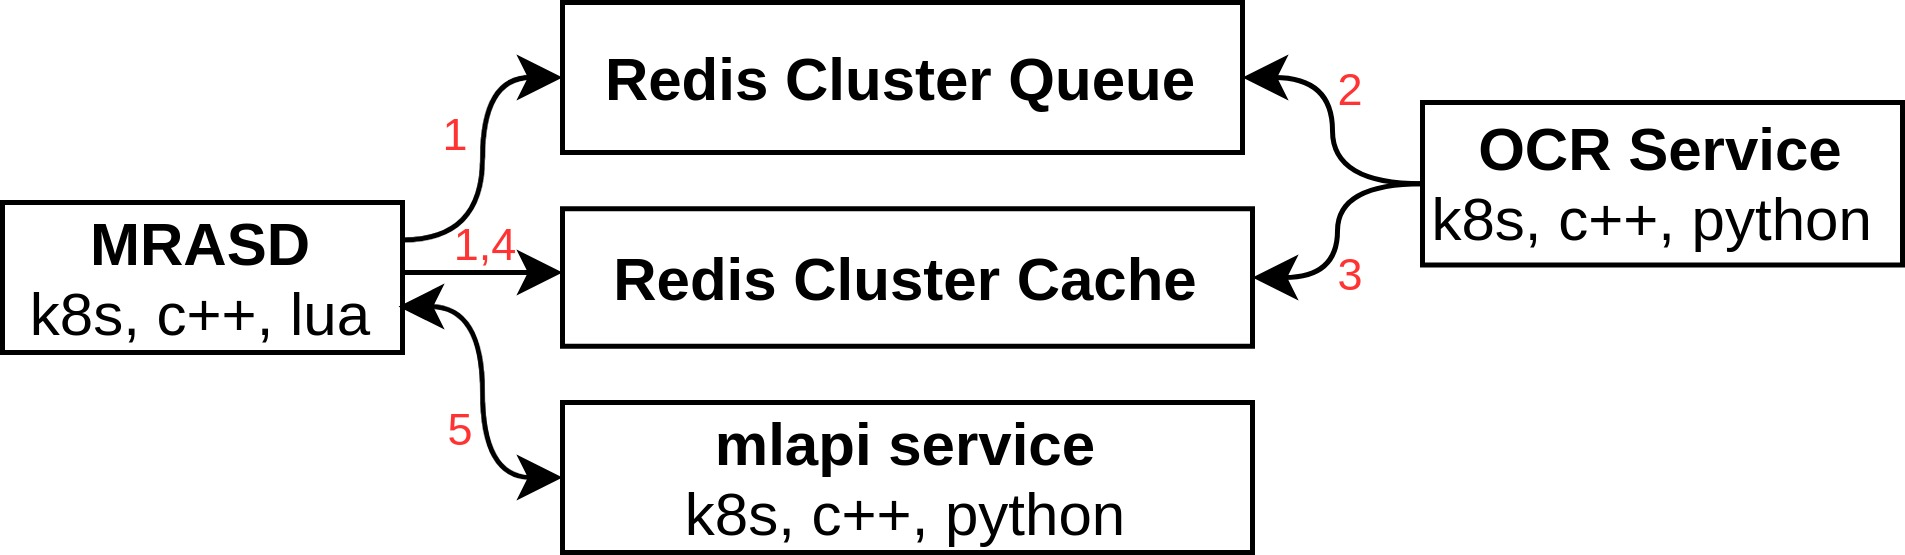
\includegraphics[width=0.8\textwidth]{images/deploy.jpg}
	\caption{\label{fig:01} Application architecture.}
\end{figure}

%%<<<<<<< HEAD
%\begin{figure}[h!]
%	\center
%	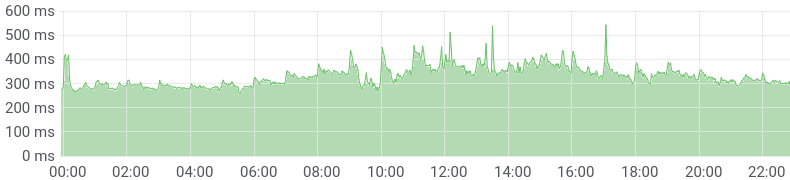
\includegraphics[width=0.8\textwidth]{images/timings_upd.png}
%	\caption{\label{fig:02} Average email processing time}	
%\end{figure}
% 
%\begin{figure}[h!]
%	\center
%	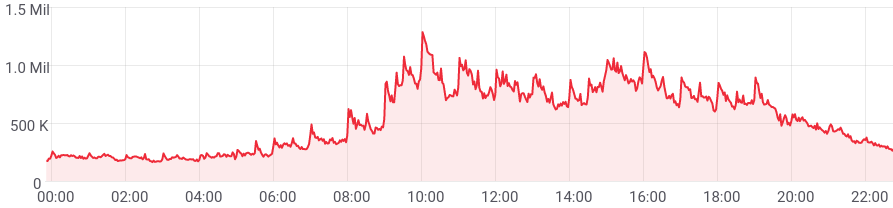
\includegraphics[width=0.95\textwidth]{images/processed_messages.png}
%	\caption{\label{fig:03} Average number of requests per minute from one of the farms}
%%=======

\begin{figure}[b]
\centering

\begin{tikzpicture}

    \node (image) at (0,0) {
        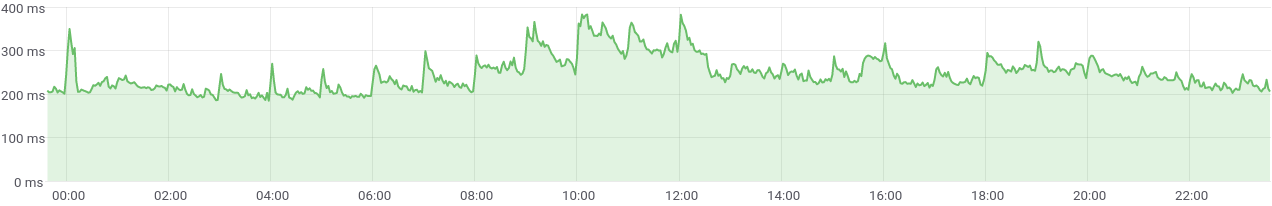
\includegraphics[width=0.99\textwidth]{images/timings1.png}
    };

    \draw [opacity=0.5] (0, -1.6) node {time in hours};

    \draw [opacity=0.5] (-8.15, 0) node {\rotatebox{90}{request time}};

\end{tikzpicture}

\caption{\label{fig:02} Average email processing time.}

\end{figure}

Since the service must operate under high loads, it is important to provide a robust architecture in which the failure of one component does not lead to the degradation of the entire system. The following client--server architecture is shown in figure\,\ref{fig:01}. Antispam daemon (mrasd) parses incoming messages and extracts text, images, and files from there. Since nested images and documents often contain junk data, it is also necessary to extract text from them. Then, documents are sent to the optical character recognition (OCR) service via a deferred redis queue (arrow 1,2), which extracts the text and stores the result in the redis cache (arrow 3).
Since, highly likely the letter can be duplicated (for example, in the case of a ddos attack or offline rechecking), in order not to load the OCR service once again, the primary check of the redis cache (arrow 1,4) is performed for the presence of already processed data for the specified document hash.
After full text extraction, the mrasd service performs all the steps of text preprocessing (reduction to a single register, removal of stop words, normalization), and then sends the text to the mlapi service (arrow 5) via the grpc protocol to vectorize the text using fast text and further obtain the FCNN prediction of the model by which a decision is made about the ``undesirability'' of the incoming message.
The proposed architecture is fairly robust because when the OCR of one (or several) instances of redis cluster fails, the entire system as a whole does not degrade.
 
\begin{figure}
\centering

\begin{tikzpicture}

    \node (image) at (0,0) {
        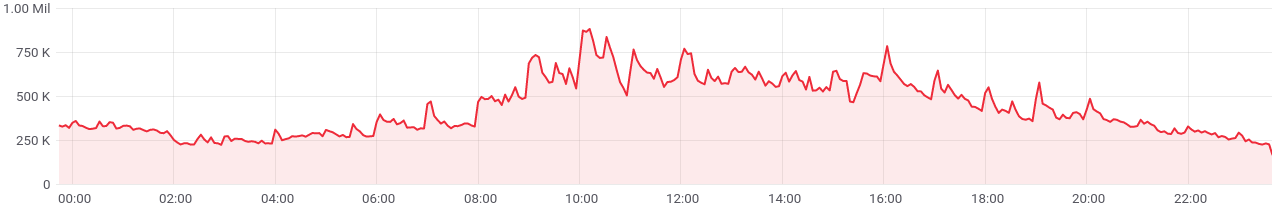
\includegraphics[width=0.99\textwidth]{images/processed_messages1.png}
    };

    \draw [opacity=0.5] (0, -1.6) node {time in hours};

    \draw [opacity=0.5] (-8.15, 0) node {\rotatebox{90}{request per minute}};

\end{tikzpicture}

\caption{\label{fig:03} Average number of requests per minute from one of the farms.}

%>>>>>>> b4a7605f38c293c05327fdf168e9f6fdc80b94a3
\end{figure}

\subsubsection*{Brief review of the libraries.}
Since services require high performance, the C++ language (stl 17, grpc, boost) is chosen as one of the most productive modern languages. Python 3 language and pyTorch framework were utilized for data analysis and training due to the high efficiency and the possibility of conducting parallel calculations, both on the CPU and on the GPU cores of the machine.
The fault tolerance of microservices is ensured by their deployment in the kubernetes (k8s) cluster, since if any pod falls for any reason. The requests are evenly balanced across the remaining live feeds, until the cluster independently returns to its previous state. 

\section{Conclusions}

The results obtained during the training of the model on real--life streaming data of users are introduced. Based on these data, one can realize that FCNN model based on Fast Text embeddings has higher classification accuracy rather then method of classical logistic regression and FCNN  model based on a bag of words.

A high--performance fault--tolerant microservice architecture is presented, which is able to withstand an average of more than $10^6$ requests per minute. The developed solution is robust. Thus, the degradation of a specific component, machine, or data center does not lead to complete inactivity of the application.

\section*{References}
\begin{thebibliography}{99}
\bibitem{Makkar2021} 
Aaisha M, Uttam G, Pradip K S
2021 {Artificial intelligence and edge computing--enabled
	web spam detection for next generation IoT
	applications} {\it IEEE Sensors Journal} {\bf } pp 1--9

\bibitem{Taylor2020}
Taylor O E, Ezekiel P S
2020 {A model to detect spam email using support vector classifier and random forest classifier} 
\emph{Int. J. Comput. Sci. Math. Theory} {\bf 6} 1 pp 1--11

\bibitem{Garg2021}
Pranjul G, Nancy G
2021 {A systematic review on spam filtering techniques based on
natural language processing framework} \emph{2021 11th International Conference on Cloud Computing, Data Science \& Engineering (Confluence 2021)} pp 30--35

\bibitem{Parmar2020}
Nandan P, Ankita S, Harshita J, Amol K K
2020 {Email spam detection using naïve Bayes and particle swarm optimization} \emph{Int. J. Inn. Res. Tech.} {\bf 6} 10 pp 367--373

\bibitem{Mohammad2020}
Mohammad RMA
2020 \emph{A lifelong spam emails classification model}
\emph{Appl. Comp. and Inf.} pp 1--20

\bibitem{Mikolov2013} 
Mikolov T, Chen K, Corrado G, and Dean J
2013 {Efficient estimation of word representations in vector space} 
arXiv:1301.3781v3

\bibitem{Bojanowski2017} 
Bojanowski P, Grave E, Joulin A, and Mikolov T
2017 {Enriching word vectors with subword information} 
arXiv:1607.04606v2

\bibitem{Bommannavar2014}
Bommannavar P, Kolcz A, Rajaraman A
2014 {Recall estimation for rare topic retrieval from large corpuses}
\emph{2014 IEEE International Conference on Big Data}

\bibitem{Yang2014}
Yang S, Kolcz A, Schlaikjer A, and Gupta P
2014 {Large--scale high-precision topic modeling on twitter} 
\emph{Proceedings of the 20th ACM SIGKDD international conference on Knowledge discovery and data mining} pp 1907--1916

\bibitem{Churikov2004} Churikov D V 2004
{Atomic functions and combined algorithm of image filtration in conditions of high intensity noise}
\emph{Radiotekhnika} \textbf{9} pp 69--71. In Russian.

\bibitem{Kravchenko2005}
Kravchenko V F, Fedorov I V, Churikov D V and Rvachev V L 2005 
{R--functions and the atomic functions in problems of complex--shaped contour objects description and digital image processing}
\emph{EW \& ES} \textbf{10} (7) pp 70--80. In Russian.

\end{thebibliography}



\end {document}
